\section{Stato dell'arte}
\label{sec:stato-arte}
In questa sezione verrà descritto lo stato dell'arte dei modelli di evacuazione da tsunami, senza focalizzarsi sui modelli di inondazione.
Successivamente alcuni lavori verranno approfonditi nelle sottosezioni seguenti,
in particolare \textcite{wang2016agent} non verrà descritto in quanto è stato scelto
come modello base per questo lavoro è verrà trattato nel capitolo apposito.

I primi modelli di evacuazione da tsunami sono stati basati sui modelli network-based utilizzati per l'evacuazione da altri disastri come
uragani, incendi e inondazioni \parencite{usuzawa1997development, imamura2001development}.

Uno dei primi aspetti che è stato preso in considerazione è il comportamento umano,
in particolare le reazioni dei residenti all'arrivo dello tsunami
e il tempo che ci mettono per iniziare a evacuare.

Queste informazioni sono state raccolte tramite dei questionari rivolti ai residenti
e usate per stimare i tempi di partenza dell'evacuazione \parencite{imamura2001development, saito2004simulation}.

Questi primi modelli network-based hanno usato come regola di \textit{path finding}
proseguire verso il nodo con altitudine maggiore.
Successivamente si è passati a usare il percorso
più breve \parencite{katada2004disaster} e altre strategie di routing basate sull'apprendimento 
come Nash equilibrium e system optimal \parencite{lammel2009towards}.

\textcite{lammel2010emergency} hanno introdotto un modello network-based che utilizza Nash equilibrium e in cui ad ogni link viene assegnata una coda FIFO,
limitata nel flusso in uscita (\textit{flow capacity}) e nella capacità di pedoni al suo interno (\textit{storage capacity}).
La velocità dei pedoni varia in base alla densità e alla \textit{flow capacity}.

Un altro aspetto importante per l'evacuazione è la conoscenza dell'ambiente da parte degli agenti.
Alcuni lavori hanno distinto gli agenti in base alla loro conoscenza e
studiato gli effetti di diverse proporzioni tra categorie di agenti.
\textcite{nguyen2012simulation} hanno definito \textit{fox agent} un pedone ben informato che segue i segnali
stradali fino a un rifugio e \textit{sheep agent} un pedone che non sa
come comportarsi e quindi segue i \textit{fox agent} o si muove casualmente.
\textcite{takabatake2017simulated} invece hanno distinto gli agenti in residenti e visitatori.
I residenti sono agenti che conoscono il percorso più breve per evacuare, mentre i visitatori
seguono gli altri scegliendo la strada con più individui o si muovono verso una zona più elevata.

Con l'aumento della potenza di calcolo è stato possibile passare da modelli network-based a modelli grid-based e ibridi.
Inoltre è stato possibile usare una quantità di dati maggiore e sfruttare il calcolo parallelo \parencite{wijerathne2013hpc, makinoshima2018enhancing}.

\textcite{wijerathne2013hpc} hanno proposto un modello grid-based che utilizza un sistema di navigazione basato
sulla visione. Gli agenti si muovono verso un luogo sicuro ben visibile scegliendo la strada con una maggiore distanza di visione.
%
Anche in questo lavoro vengono distinti visitatori, che si affidano alla visione, e non-visitatori, che hanno conoscenza di un'area
limita al di fuori della quale vengono considerati visitatori.

% Un altro modello grid-based è quello di \textcite{mas2012agent} 
% in cui è stato proposto un modello di evacuazione statica che da un insieme di informazioni % TODO: specificare (dati demografici, morfologia del terreno, distribuzione della popolazione, ...)
% calcola una mappa dei tempi di evacuazione

% Altri lavori hanno analizzato come i tempi di partenza influenzano il tempi di evacuazione e il numero di vittime
% \parencite{wang2016agent, takabatake2017simulated}.

% Successivamente i modelli di evacuazione da tsunami si sono concentrati sulle applicazioni come trovare delle contromisure, 
% il miglioramento delle modalità di evacuazione
% tramite l'analisi delle congestioni del traffico, il posizionamento dei rifugi e lo scambio di informazioni durante l'evacuazione.
% \parencite{taubenbock2013risk} %TODO: aggiungere citazioni

In molti modelli vengono considerati esclusivamente solo pedoni, ma alcuni lavori hanno analizzato l'aggiunta della presenza di auto e altri veicoli,
e si concentrano nella gestione delle interazioni tra i diversi tipi di agenti.

\textcite{goto2012tsunami} hanno considerato gli individui raggruppati in famiglie e categorizzato le famiglie in:
pedoni lenti, pedoni normali, motociclisti e occupanti di un'auto, gestendo le loro velocità in base alla densità e inoltre hanno
modellato le interazioni dei diversi agenti all'interno di una corsia stradale.

\textcite{wang2016agent} hanno proposto un modello in cui auto e pedoni evacuano separatamente e vengono gestite esclusivamente interazioni auto-auto. Ai pedoni viene assegnata
una velocità costante tramite una distribuizione normale che comprende diversi range di velocità dei pedoni.

\textcite{wang2021novel} hanno ripreso il lavoro di \textcite{wang2016agent} e, 
ispirandosi al lavoro \textcite{goto2012tsunami}, modificato la gestione delle interazioni proponendo un modello in cui sia pedoni che auto hanno una velocità variabile in base alla densità.
Vengono distinti diversi stati di traffico in base al rapporto tra il volume dei pedoni e delle auto: \textit{vehicle-dominated}, \textit{balanced}, e \textit{pedestrian-dominated}. 
Inoltre per rendere il modello più realistico sono stati considerati i danni sulla rete stradale causati dal terremoto che si verifica prima dello tsunami.


\subsection{lammel2010emergency}
Questo lavoro utilizza un modello network-based per simulare un'evacuzione in larga scala di 450,000 pedoni.

All'inizio della simulazione tutti gli agenti siano nelle loro abitazioni 
e inizino ad evacuare dopo un certo tempo di partenza individuale.

I pedoni evacuano seguendo il percorso più breve e per alcuni di essi viene effettuato un \textit{re-planning} del percorso tramite Nash equilibrium,
considerando i tempi di attraversamento sulle strade.

La simulazione del traffico è implementata con un sistema a code dove ad ogni link viene assegnata una coda FIFO, 
limitata nel flusso in uscita \textit{flow capacity} e nella capacità di pedoni al suo interno \textit{storage capacity}.

La velocità viene aggiornata tramite la relazione $v = \min[v_{max}, FC / D]$, dove $v$ la velocità,
$V_{max}$ la velocità massima, $D$ la densità e $FC$ è la \textit{flow capacity}.
%
Inoltre è stata considerata una velocità massima di 1.66 m/s per considerare il
flusso dei pedoni in caso di emergenza.

\newpage


\subsection{goto2012tsunami}
Una popolazione di 80,000 individui è stata considerata.
Gli agenti evacuano seguendo il percorso più breve verso nove possibili rifugi, alcuni dei quali con una capacità limitata.

\vspace*{5mm}

Sono stati considerati diversi scenari in base al tempo di partenza, al numero di auto e di pedoni,
o alla possibilità di cambiare la destinazione nel caso il rifugio sia pieno.

\vspace*{5mm}

Un agente colpito dallo tsunami muore quando la profondità dello tsunami supera 1m.

\vspace*{5mm}

In questo lavoro diversi tipi di agenti sono modellati pedoni, motocicli e auto,
dove ogni agente rappresenta una famiglia.

\vspace*{5mm}

I pedoni sono suddivisi i pedoni normali con una velicità massima di 1.5 m/s,
mentre i pedoni lenti sono famiglie con handicap, infanti o anziani con una velocità massima di 0.75 m/s.
le velocità sono ridotte all'aumentare della densità fino ad un massimo di 6 $p/m^2$.

\vspace*{5mm}

Per i motocicli una velocità massima di 30km/h è stata considerata con una densità massima di 0.9 $p/m^2$.

\vspace*{5mm}

Le auto in assenza di ostacoli si muovono per $L_{f} = V_{f} x \Delta_{t} $, dove $L_{f}$ è la \textit{free run length},
$V_{f}$ la \textit{free run speed} e $\Delta_{t}$ il \textit{time step}.
La velocità cambia in base alla densità in fronte con un valore massimo di free run speed di 40 km/h.

\vspace*{5mm}

In caso di più corsie se una corsia è vuota in base alla density ahead l'auto allora può cambiare corsia,
per i pedoni e motocicli se la density ahead supera 1 $p/m^2$ occupano la corsia successiva sulla sinistra.

\vspace*{5mm}

In questo lavoro la densità in un'area davanti viene definita tramite la seguente formula
$\rho = n /(L \times W)$, dove $n$ è il numero di agenti nell'area $L \times W$, $L$ è la lunghezza di ricerca, 
che assume valori di 3m per i pedoni e 16.7m per i motocicli, e $W$ la larghezza della strada.
Per le auto la densità invece è definita nel seguente modo $\rho = n /((W - W_{c}) x L_{f})$, dove $W_{c}$ è la larghezza di un auto.

\vspace*{5mm}

Nel calcolo della densità un auto viene considerata 10 volte un pedone ed un motociclo 2 volte.
nel caso di interruzioni del traffico devono o aspettare o seguire il secondo shortest path.

\begin{figure}[ht]
    \centering
    \begin{subfigure}{0.45\textwidth}
        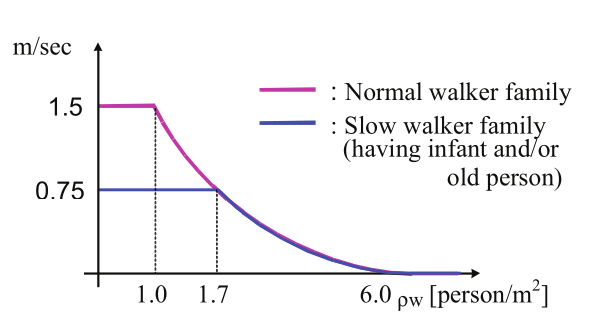
\includegraphics[width=\textwidth]{images/speed_GOTO.png}
        \caption{}
        \label{fig:adaads}
    \end{subfigure}
    \begin{subfigure}{0.45\textwidth}
        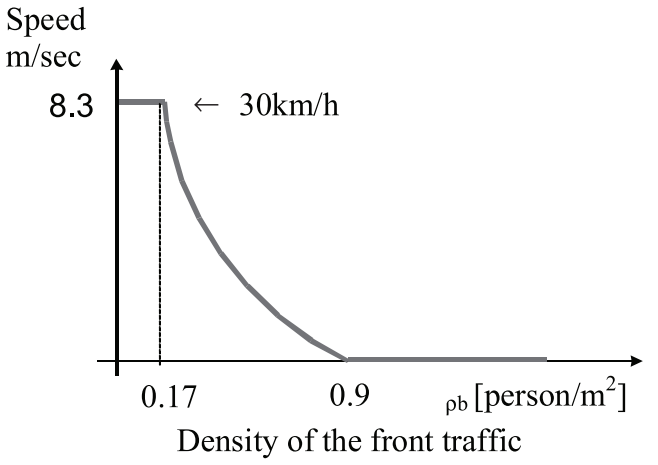
\includegraphics[width=\textwidth]{images/speed_GOTO_motocicli.png}
        \caption{}
        \label{fig:ssadada}
    \end{subfigure}
    \begin{subfigure}{0.45\textwidth}
        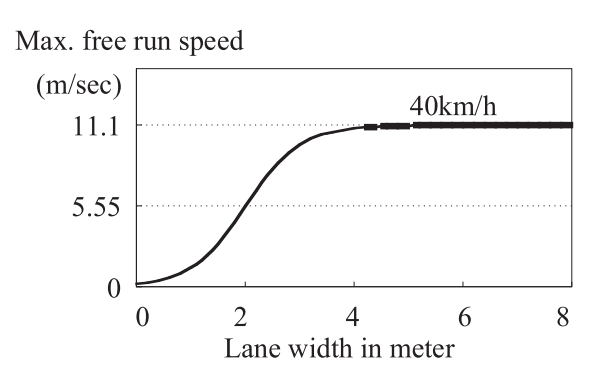
\includegraphics[width=\textwidth]{images/speed_GOTO_auto.png}
        \caption{}
        \label{fig:wrsnjds}
    \end{subfigure}
    \caption{Relazione velocità-densità: a) per i pedoni, b) motocicli e c) auto}
    \label{fig:ankdasndk}
\end{figure}


\subsection{takabatake2017simulated}
In questo lavoro è stato sviluppato un modello di evacuazione da tsunami che considera
21,238 pedoni distinti tra residenti e visitatori.

I residenti si assume che conoscano il percorso più breve
per il rifugio più vicino dal punto in cui si trovano all'inizio dell'evacuazione.
%
I visitatori invece seguono due regole adottando un approccio probabilistico:
\begin{itemize}
    \item “following other individuals”: ad ogni intersezione seguono la strada con più individui.
    \item “going to higher ground”: ad ogni intersezione scelgono la strada che porta a un altezza maggiore.
\end{itemize}

Sia i residenti che i visitatori vengono distinti in base all'età con una velocità massima di 1.19 m/s (Under 65) e 0.96 m/s (Over 65).
Basandosi sul lavoro di \textcite{older1968movement} hanno assunto una decrescità lineare della 
velocità da un livello di densità di 0.3 p/m² a uno di 3.0 p/m² (Fig. \ref{fig:speed-linear}).

\begin{figure}[ht]
    \centering
    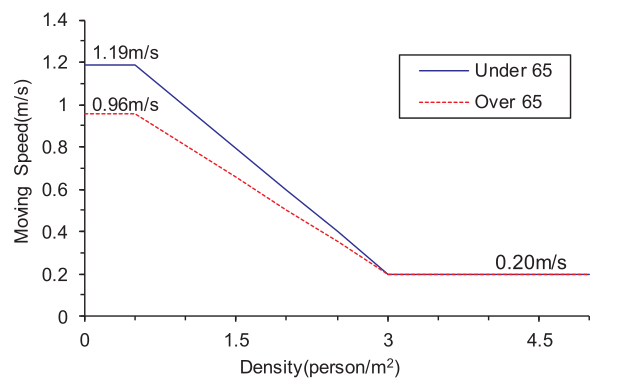
\includegraphics[width=0.7\textwidth]{images/speed_Linear.png}
    \caption{Relazione velocità-densità \textcite[]{takabatake2017simulated}}
    \label{fig:speed-linear}
\end{figure}

Per quanto riguarda i tempi di partenza sono stati usati due approcci sia per residenti che visitatori:
\begin{itemize}
    \item ``all-togheter'': gli agenti evacuano allo stesso tempo.
    \item ``delayed evacuation'': il tempo di partenza degli agenti viene assegnato secondo la distribuzione di Rayleigh.
\end{itemize}

I rifugi prevedono una capacità limitata. Quando un agente arriva in un rifugio già pieno si dovrà dirigere a un altro rifugio.
Per i visitatori viene applicato un delay di 30 secondi per chiedere informazioni sulla posizione del rifugio più vicino.

Il casualty model utilizzato considera che un agente muore quando l'altezza delle onde nella sua posizione supera i 0.3 m.


\subsection{Z. Wang e Jia (2021)}
In questo lavoro viene proposto un modello di evacuazione da tsunami multimodale e una valutazione dei rischi modellando l'incertezza
nei danni sismici nelle strade e in altri parametri del modello.

Sono state considerate diverse popolazioni al variare del numero di agenti: 5000 e 10000,
che rappresentano la popolazione all'inizio dell'estate e 15000 rappresenta il picco nella stagione estiva.

Gli agenti sono distinti in pedoni e auto ed evacuano verso il rifugio più vicino seguendo il percorso più breve.
Si assume che ogni auto contenga 4 agenti e che sia equivalente a 10 volte un pedone in spazio occupato.
Gli agenti per poter evacuare in auto dovranno prima raggiungere a piedi degli appositi parcheggi.

Il modello dei pedoni considera una velocità distribuita secondo una normale $\mathcal{N}(\mu_p,\sigma_p)$ troncata tra 0.75 m/s e 3.83 m/s e
con $\mu_p \sim \mathcal{U}(1.4, 2)$ e $\sigma_p \sim \mathcal{U}(0.1, 0.6)$.
Inoltre viene aggiornata in base alla densità di fronte all'agente con una \textit{search length} di 4m secondo l'andamento mostrato in figura \ref*{fig:dadknakdand}.

\begin{figure}[ht]
    \centering
    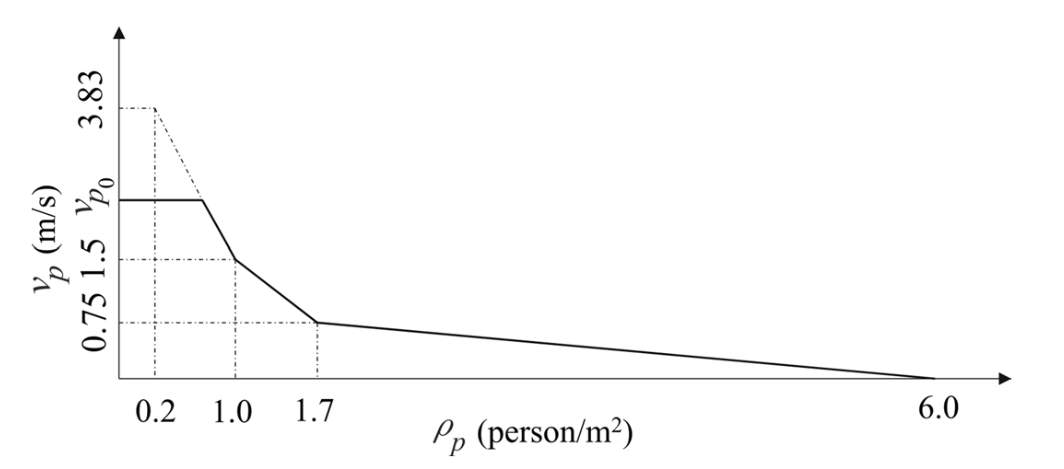
\includegraphics[width=0.7\textwidth]{images/speed_WANG.png}
    \caption{Relazione velocità-densità \textcite{wang2021novel} basato su un approssimazione del modello di \textcite{goto2012tsunami}}
    \label{fig:dadknakdand}
\end{figure}

Per le auto è stato utilizzato il modello di \textcite{greenshields1935study} che aggiorna la velocità in base alla densità di fronte lungo la \textit{free run length},
con una massima velocità di 40 km/h e una densità massima di 160 veh/km per i link senza restrizioni sul traffico date dai danni sismici, altrimenti 120 veh/km.

Per la gestione delle interazioni tra auto e pedoni vengono definite tre fasi di traffico in base al rapporto
tra il volume dei pedoni e delle auto: \textit{vehicle-dominated}, \textit{balanced} e \textit{pedestrian-dominated}.
Al variare della fase cambia la larghezza della strada occupabile sia per pedoni che per le auto.

Per i tempi di partenza viene utilizzata la distribuzione di Rayleigh dove i parametri
invece di essere fissati seguono delle apposite distribuzioni uniformi.

Rispetto ad altri lavori che utilizzano un livello di profondità fissa per determinare la morte degli agenti, in questo lavoro
viene considerato che la profondità sia distribuita uniformemente in [0.5, 3]. 
